% ===== Part 1 = chapter 1, Mind controls (~42 min) =====
\partopener{Մաս 1 · Գլուխ 1}{Մարմնի կառավարում}{Ինչպես է ուղեղը ղեկավարում մարմինը (ու սովորաբար խառնում ամեն ինչ)}{panic}{mint}

% Chapter opening joke: the brain's first job was keeping the body alive
\begin{frame}{Սկզբում ուղեղը մեկ գործ ուներ}
  \begin{columns}[c]
    \begin{column}{0.56\textwidth}
      \begin{bookquote}
        Ցամաք դուրս եկած առաջին ձուկը չէր տանջվում կասկածներով. «Ինչու՞ եմ սա անում։ Այստեղ չեմ կարողանում շնչել, ու ոտքեր էլ չունեմ, ինչ էլ որ դրանք լինեն։ Վերջին անգամն եմ Գարիի հետ "ճիշտ թե համարձակություն" խաղում»։
      \end{bookquote}
    \end{column}
    \begin{column}{0.38\textwidth}
      \centering
      \bigemoji[1.6cm]{fish}\par\medskip
      \onslide<2->{%
      \begin{card}[colback=mint!35!cardwhite]
        Մտածելը հետո եկավ։ Ուղեղի գլխավոր գործը մարմինը \textbf{ողջ պահելն} էր՝ ամեն գնով։
      \end{card}}
    \end{column}
  \end{columns}
  \vspace{4mm}
  \onslide<3->{\centering Լեզուն ու տրամաբանությունը քիչ բան արժեն, եթե մոռանում ես ուտել կամ ընկնում ես ժայռից։\par}
\end{frame}

% The two bosses in one head
\begin{frame}{Երկու պետ մեկ գլխում}
  \begin{columns}[T]
    \begin{column}{0.47\textwidth}
      \begin{card}[colback=mint!35!cardwhite]
        \emoji[1.4em]{lizard}\ {\blackfont «Սողունի ուղեղ»}\par\smallskip
        Շնչառություն, սիրտ, քուն։ Համառ գործընկերը, որ գրամեքենա է պահանջում. «միշտ այսպես ենք արել»
      \end{card}
    \end{column}
    \begin{column}{0.47\textwidth}
      \onslide<2->{%
      \begin{card}[colback=lavender!40!cardwhite]
        \emoji[1.4em]{boss}\ {\blackfont Նոր կեղև} (neocortex)\par\smallskip
        Գիտակցություն, տրամաբանություն։ Նոր պետը, որ ոչինչ չգիտի, բայց ամեն ինչ հրահանգում է
      \end{card}}
    \end{column}
  \end{columns}
  \vspace{3mm}
  \onslide<3->{%
  \begin{scienceupdate}
    Այս բաժանումը (triune brain) պարզեցում է. ուղեղի մասերը միասին են էվոլյուցիա անցել։
  \end{scienceupdate}}
\end{frame}

% ---------------------------------------------------------------- motion sickness
\topicopener{rollercoaster}{Ծովախտ}{Կանգնեցրե՛ք գիրքը, ես իջնում եմ}{Ինչու է ճանապարհին սիրտդ խառնում}{sick}

\begin{frame}{Շարժվելը կենսական է. ինչու՞ է այն սիրտ խառնում}
  \begin{columns}[c]
    \begin{column}{0.5\textwidth}
      \begin{poll}
        \emoji{car}\,\emoji{ship}\,\emoji{airplane}\par\smallskip
        Բարձրացրու ձեռքդ Zoom-ում, եթե քեզ երբևէ մեքենայում, ավտոբուսում կամ նավում վատ է եղել։
      \end{poll}
    \end{column}
    \begin{column}{0.44\textwidth}
      \onslide<2->{%
      \begin{itemize}
        \item Մարդը քայլելու համար է ստեղծված
        \item Միլիոնավոր տարիներ շարժվել ենք, ու դա մեզ փրկել է
        \item Ուրեմն ինչու՞ է ուղեղը շարժումից \textbf{փսխելու} որոշում կայացնում
      \end{itemize}}
    \end{column}
  \end{columns}
  \vspace{4mm}
  \onslide<3->{%
  \begin{card}[colback=brainpink!25!cardwhite]
    \centering Մեղավորը ստամոքսը չէ, այլ \textbf{ուղեղը}։ Ու ծովախտ (motion sickness) լինում է միայն \textbf{տրանսպորտում}։
  \end{card}}
\end{frame}

\begin{frame}{Ինչպես ենք զգում շարժումը}
  \begin{columns}[T]
    \begin{column}{0.31\textwidth}
      \begin{card}[fontupper=\footnotesize]
        \emoji[1.4em]{walking}\ {\blackfont Ողնուղեղը}\par\smallskip
        «Ռիթմ գեներատորները» քայլում են մեր փոխարեն՝ առանց ուղեղի
      \end{card}
    \end{column}
    \begin{column}{0.31\textwidth}
      \onslide<2->{%
      \begin{card}[fontupper=\footnotesize]
        \emoji[1.4em]{hand}\ {\blackfont Պրոպրիոցեպցիա}\par\smallskip
        Զգում ես մարմնիդ մասերի դիրքը առանց նայելու
      \end{card}}
    \end{column}
    \begin{column}{0.31\textwidth}
      \onslide<3->{%
      \begin{card}[fontupper=\footnotesize]
        \emoji[1.4em]{ear}\ {\blackfont Ներքին ականջը}\par\smallskip
        Հեղուկով խողովակներ (vestibular system)՝ դիրքի ու արագացման սենսոր
      \end{card}}
    \end{column}
  \end{columns}
  \onslide<2->{%
  \begin{tryit}
    Մատներդ շարժիր մեջքիդ հետևում. չես տեսնում, բայց գիտես ժեստը։
  \end{tryit}}
\end{frame}

\begin{frame}{Աչքերն ու ականջը վիճում են}
  \centering
  % Motion sickness as a sensory conflict: eyes vs inner ear -> confused
% old brain -> "poison!" -> vomit. Reveals in 5 steps (use inside a frame).
\begin{tikzpicture}[
    msg/.style={draw=#1, line width=1pt, fill=#1!8!cardwhite, rounded corners=3mm,
                text width=4.1cm, align=left, inner sep=5pt, font=\small},
    lbl/.style={fill=#1, text=white, font=\blackfont\small, rounded corners=1.5mm, inner sep=3pt},
    sig/.style={-{Stealth[length=3mm]}, line width=1.6pt, #1},
  ]
  \path[use as bounding box] (-7.2,-2.9) rectangle (7.2,3.0);

  % --- the car with a reader inside --------------------------------------
  \begin{scope}[shift={(-4.6,-1.25)}]
    \draw[plum!50, line width=1pt] (-2.4,-0.95) -- (2.6,-0.95);              % road
    \foreach \y in {0.15,-0.2,-0.55}{\draw[plum!40, line width=1pt, line cap=round] (-2.55,\y) -- (-2.05,\y);}
    \filldraw[fill=lavender, draw=plum, line width=1pt, rounded corners=3mm]
      (-1.9,-0.6) -- (-1.9,0.15) -- (-1.15,0.3) -- (-0.7,1.05) -- (0.95,1.05) -- (1.5,0.3)
      -- (2.2,0.2) -- (2.2,-0.6) -- cycle;
    \filldraw[fill=cardwhite, draw=plum, line width=0.8pt, rounded corners=1.5mm]
      (-0.95,0.32) -- (-0.6,0.9) -- (0.85,0.9) -- (1.25,0.32) -- cycle;
    \fill[plum] (0.05,0.62) circle (0.17);                                    % head
    \filldraw[fill=amOrange, draw=plum, line width=0.6pt, rotate around={-25:(0.45,0.5)}]
      (0.35,0.38) rectangle (0.6,0.66);                                       % book
    \foreach \x in {-1.15,1.45}{
      \filldraw[fill=plum, draw=plum] (\x,-0.6) circle (0.36);
      \fill[cardwhite] (\x,-0.6) circle (0.13);
    }
    \node[font=\mediumfont\small, text=plum] at (0.15,-1.3) {կարդում ես հետևի նստարանին};
  \end{scope}

  % --- eyes ----------------------------------------------------------------
  \node[msg=amBlue, visible on=<2->] (eye) at (-4.6,1.9)
    {«Գիրքն անշարժ է, նստարանն անշարժ է։ \textbf{Մենք չենք շարժվում}»};
  \node[lbl=amBlue, visible on=<2->, anchor=south west] at ([xshift=3mm, yshift=-1mm]eye.north west)
    {\emoji[1em]{eye}\ աչքեր};

  % --- inner ear -----------------------------------------------------------
  \node[msg=amOrange, visible on=<3->] (ear) at (0,1.9)
    {«Արագացում, արգելակ, շրջադարձ։ \textbf{Մենք արագ շարժվում ենք}»};
  \node[lbl=amOrange!85!black, visible on=<3->, anchor=south west] at ([xshift=3mm, yshift=-1mm]ear.north west)
    {\emoji[1em]{ear}\ ներքին ականջ};

  % --- the brain gets both -------------------------------------------------
  \pic[scale=0.8, visible on=<4->] at (4.6,0.0) {noggin=confused};
  \draw[sig=amBlue, visible on=<4->] (eye.south east) to[out=-20, in=170] (3.4,0.2);
  \draw[sig=amOrange!85!black, visible on=<4->] (ear.south east) to[out=-30, in=120] (3.85,1.0);
  \node[say, visible on=<4->, callout absolute pointer={(4.9,1.1)}, text width=3.1cm, font=\handfont\normalsize]
    at (5.6,2.4) {Սրանք իրար չեն համընկնում։ Ներսում ինչ-որ բան լուրջ խառնվել է...};

  % --- conclusion ----------------------------------------------------------
  \node[visible on=<5->, draw=pinkdark, line width=1.5pt, fill=blush!20!cardwhite, rounded corners=3mm,
        text width=4.6cm, align=center, inner sep=6pt, font=\small] (poison) at (4.6,-2.15)
    {{\blackfont\color{pinkdark} Հին ուղեղ՝ «Սա ԹՈՒՅՆ է»}\\ \emoji{vomit}\ Արտակարգ պլան՝ դատարկել ստամոքսը};
  \draw[sig=pinkdark, visible on=<5->] (4.6,-1.15) -- (poison.north);
\end{tikzpicture}

\end{frame}

\begin{frame}{Հին ուղեղի տրամաբանությունը}
  \begin{columns}[c]
    \begin{column}{0.56\textwidth}
      \centering
      \begin{meme}[6.8cm]{is_this_a_pigeon.jpg}
        \memecap{0.36}{0.55}{սողունի ուղեղ}
        \memecap{0.84}{0.95}{մեքենայով երթևեկ}
        \memecap[font=\blackfont\large]{0.5}{0.08}{Սա թո՞ւյն է}
      \end{meme}
    \end{column}
    \begin{column}{0.4\textwidth}
      \onslide<2->{%
      \begin{bookquote}
        Բնության մեջ միայն թույնը կարող է այդքան խառնել ներքին համակարգերը։ Իսկ թույնի դեմ կա մեկ խելամիտ պատասխան՝ դուրս հանել այն, ու շտապ։
      \end{bookquote}}
    \end{column}
  \end{columns}
\end{frame}

\begin{frame}{Ինչու է ծովում ամենավատը}
  \begin{columns}[T]
    \begin{column}{0.5\textwidth}
      \begin{itemize}
        \item Ցամաքում ծառերն ու շենքերը անցնում են կողքովդ, ու աչքերը տեսնում են շարժումը
        \item Ծովում միայն ջուր է ու հեռավոր հորիզոն. աչքերը պնդում են՝ \textbf{չենք շարժվում}
        \item Իսկ ալիքները անկանխատեսելի վեր-վար են անում, ու ներքին ականջը գժվում է
      \end{itemize}
    \end{column}
    \begin{column}{0.44\textwidth}
      \onslide<2->{%
      \begin{bookquote}
        Սփայք Միլիգանին հարցրել են, թե ինչն է լավագույն միջոցը ծովախտի դեմ։\par\smallskip
        Պատասխանը՝ \textbf{«Նստիր ծառի տակ»}։
      \end{bookquote}
      \centering\bigemoji[1.3cm]{tree}}
    \end{column}
  \end{columns}
\end{frame}

\begin{frame}{Ինչն է օգնում (նույն տրամաբանությամբ)}
  \begin{columns}[T]
    \begin{column}{0.5\textwidth}
      \begin{card}[colback=mint!35!cardwhite]
        \begin{itemize}
          \item Նայիր պատուհանից, \textbf{հորիզոնին}. աչքերը կհամաձայնվեն ականջի հետ
          \item Նստիր առջևում, որտեղից ճանապարհը երևում է
          \item Ճանապարհին մի կարդա ու հեռախոսին մի նայիր
        \end{itemize}
      \end{card}
    \end{column}
    \begin{column}{0.44\textwidth}
      \onslide<2->{%
      \begin{scienceupdate}
        Սա ամենատարածված վարկածն է (sensory conflict), բայց կա նաև այլընտրանք՝ «նիստագմի վարկածը». աչքի մկանների ձգումն է գրգռում թափառող նյարդը։ Մինչև վերջ դեռ պարզ չէ։
      \end{scienceupdate}}
    \end{column}
  \end{columns}
\end{frame}

% ---------------------------------------------------------------- appetite
\topicopener{doughnut}{Ախորժակ}{Աղանդերի տեղ կա՞}{Ով է իրականում որոշում՝ երբ ու ինչքան ենք ուտում}{hungry}

\begin{frame}{Ստամոքսը սանդուղքի ամենացածր աստիճանն է}
  \begin{columns}[c]
    \begin{column}{0.5\textwidth}
      \begin{itemize}
        \item Ստամոքսը ձգվում է, նյարդերը ուղեղին ասում են՝ «կուշտ ենք»
        \item Նիհարելու կոկտեյլները հենց դա են խաբում. արագ լցնում են ստամոքսը
        \item Բայց 20 րոպեից շատերը նորից սոված են
      \end{itemize}
      \vspace{2mm}
      \onslide<2->{%
      \begin{card}[colback=peach!40!cardwhite]
        Ստամոքսի ազդանշանը երկար սանդուղքի \textbf{ամենացածր} աստիճանն է։ Սանդուղքը տանում է մինչև ուղեղ ու երբեմն պտույտներ է տալիս։
      \end{card}}
    \end{column}
    \begin{column}{0.44\textwidth}
      \centering
      \begin{tikzpicture}[rung/.style={draw=plum, line width=0.8pt, fill=cardwhite, rounded corners=2mm,
          minimum width=4.6cm, minimum height=0.56cm, font=\small, text=plum, inner sep=2pt}]
        \draw[plum, line width=1.6pt] (-2.55,-0.35) -- (-2.55,3.75) (2.55,-0.35) -- (2.55,3.75);
        \foreach \y/\t/\e/\s in {0/ստամոքսի ձգում/burger/1, 0.7/հորմոններ/drool/2, 1.4/պարգև (քաղցր)/cake/3,
                               2.1/սովորություն ու ժամ/clock12/4, 2.8/տեսք ու հիշողություն/eyes/5, 3.5/տրամադրություն/thought/6}{
          \node[rung, visible on=<\s->] at (0,\y) {\emoji[1em]{\e}\ \t};}
      \end{tikzpicture}
    \end{column}
  \end{columns}
\end{frame}

\begin{frame}{Գրելին ընդդեմ լեպտինի}
  \centering
  % Hunger tug-of-war: ghrelin (stomach, "EAT!") vs leptin (fat cells,
% "ENOUGH!"), with the brain as a referee that stops listening (slide 2).
\begin{tikzpicture}[
    tag/.style={font=\blackfont\large, text=#1},
    sub/.style={font=\small, text=plum, align=center, text width=3.2cm},
  ]
  \path[use as bounding box] (-7.1,-2.75) rectangle (7.1,3.0);

  % rope
  \draw[peachdark, line width=2.2pt, decorate,
        decoration={coil, aspect=0.35, segment length=2.4mm, amplitude=1.3mm}]
    (-4.6,-0.35) -- (4.6,-0.35);
  \fill[pinkdark] (0,-0.35) -- (0.12,-1.05) -- (-0.12,-1.05) -- cycle;      % flag
  \draw[plum!40, dashed, line width=0.8pt] (0,-1.3) -- (0,0.3);

  % --- left: the stomach (ghrelin) -------------------------------------
  \begin{scope}[shift={(-5.6,-0.35)}]
    \filldraw[fill=peach, draw=plum, line width=1pt]
      (-0.2,1.0) .. controls (0.9,1.2) and (1.1,0.2) .. (0.8,-0.4)
      .. controls (0.5,-1.1) and (-0.6,-1.2) .. (-0.95,-0.5)
      .. controls (-1.15,-0.1) and (-0.75,0.2) .. (-0.45,0.25)
      .. controls (-0.25,0.3) and (-0.45,0.85) .. (-0.2,1.0) -- cycle;
    \filldraw[fill=white, draw=plum] (0.05,0.2) circle (0.14) (0.45,0.2) circle (0.14);
    \fill[plum] (0.08,0.18) circle (0.06) (0.48,0.18) circle (0.06);
    \filldraw[fill=plum] (0.12,-0.25) .. controls (0.2,-0.5) and (0.45,-0.5) .. (0.5,-0.22) -- cycle;
    \draw[plum, line width=1.6pt, line cap=round] (0.75,0.0) -- (1.15,0.0);  % arm on rope
    \node[tag=peachdark] at (0,1.5) {Գրելին};
    \node[sub] at (0,-1.6) {արտադրում է \textbf{դատարկ ստամոքսը}};
    \node[say, callout absolute pointer={(0.3,1.85)}, font=\handfont\large] at (1.55,2.55) {ԿԵ՛Ր}; % tail ends above the label, not on it
  \end{scope}

  % --- right: the fat cell (leptin) -------------------------------------
  \begin{scope}[shift={(5.6,-0.35)}]
    \filldraw[fill=butter, draw=plum, line width=1pt] (0,0) circle (0.95);
    \filldraw[fill=amOrange!55, draw=plum!60] (0.35,0.45) circle (0.22);    % nucleus
    \filldraw[fill=white, draw=plum] (-0.45,0.1) circle (0.14) (-0.05,0.1) circle (0.14);
    \fill[plum] (-0.48,0.08) circle (0.06) (-0.08,0.08) circle (0.06);
    \draw[plum, line width=1pt, line cap=round] (-0.45,-0.35) -- (-0.05,-0.35);
    \draw[plum, line width=1.6pt, line cap=round] (-0.95,0.0) -- (-1.15,0.0);
    \node[tag=lavenderdark] at (0,1.5) {Լեպտին};
    \node[sub] at (0,-1.6) {արտադրում են \textbf{ճարպային բջիջները}};
    \node[say, callout absolute pointer={(-0.3,1.85)}, font=\handfont\large] at (-1.75,2.55) {ԲԱՎԱԿԱ՛Ն Է};
  \end{scope}

  % --- the referee ------------------------------------------------------
  \pic[scale=0.62, visible on=<2->] at (0,1.15) {noggin=smug};
  \node[say, visible on=<2->, callout absolute pointer={(0,0.2)}, text width=4.0cm, font=\handfont\small]
    at (0,-2.05) {Ամեն օր նույն ազդանշանները... Վաղուց չեմ լսում։ Ի դեպ, էն տո՞րթ է};
\end{tikzpicture}

\end{frame}

\begin{frame}{Ինչու՞ աղանդերի համար միշտ տեղ կա}
  \begin{columns}[c]
    \begin{column}{0.42\textwidth}
      \begin{itemize}
        \item Կերել ես կես կով կամ մի կաթսա պանրով մակարոն, բայց աղանդերը դեռ «տեղավորվում է»
        \item<2-> Ստամոքսն ասում է՝ «տեղ չկա»
        \item<3-> Ուղեղը քաղցրը համարում է \textbf{պարգև} ու ուղղակի անտեսում է ստամոքսի կարծիքը
      \end{itemize}
    \end{column}
    \begin{column}{0.54\textwidth}
      \centering
      \onslide<4->{%
      \begin{meme}[7cm]{distracted_boyfriend.jpg}
        \memecap{0.25}{0.32}{աղանդեր}
        \memecap{0.58}{0.62}{ուղեղ}
        \memecap{0.86}{0.38}{«կուշտ եմ»\\ ստամոքս}
      \end{meme}}
    \end{column}
  \end{columns}
\end{frame}

\begin{frame}{Հին ուղեղ ընդդեմ նորի. 1 : 1}
  \begin{columns}[T]
    \begin{column}{0.47\textwidth}
      \begin{card}[colback=mint!35!cardwhite]
        \centering
        \emoji[1.6em]{rollercoaster}\par\smallskip
        {\blackfont\large Ծովախտ}\par\smallskip
        Հաղթում է \textbf{հին} ուղեղը \emoji{lizard}\par
        նոր կեղևը գիտի, որ թույն չկա, բայց հին ուղեղը չի լսում
      \end{card}
    \end{column}
    \begin{column}{0.47\textwidth}
      \onslide<2->{%
      \begin{card}[colback=lavender!40!cardwhite]
        \centering
        \emoji[1.6em]{icecream}\par\smallskip
        {\blackfont\large Աղանդեր}\par\smallskip
        Հաղթում է \textbf{նոր} ուղեղը \emoji{boss}\par
        ստամոքսն ասում է «բավ է», բայց կեղևը որոշում է, որ պարգևն ավելի կարևոր է
      \end{card}}
    \end{column}
  \end{columns}
  \vspace{4mm}
  \onslide<3->{\centering\mascot[1.4cm]{smug}\par}
\end{frame}

\begin{frame}{Մի տորթ, որ փչացրեց ամեն ինչ}
  \begin{columns}[c]
    \begin{column}{0.56\textwidth}
      \begin{itemize}
        \item Տարիներով տորթ ես կերել առանց խնդրի
        \item<2-> Մի օր տորթից հետո վատացար։ Գուցե կրեմն էր փչացած, գուցե \textbf{բոլորովին այլ պատճառով}
        \item<3-> Ուղեղն այլևս թույլ չի տալիս։ Միայն նայելուց սիրտդ խառնում է (taste aversion)
        \item<4-> Զզվանքը էվոլյուցիայի պաշտպանությունն է թունավոր ու փչացած սննդից, ու այն շատ դժվար է «ջնջել»
      \end{itemize}
    \end{column}
    \begin{column}{0.38\textwidth}
      \centering
      \bigemoji[1.4cm]{cake}\ \raisebox{0.4cm}{\Large$\rightarrow$}\ \bigemoji[1.4cm]{nauseated}\par\medskip
      \onslide<5->{%
      \begin{chatbox}
        Կա՞ ուտելիք, որ այլևս չես կարողանում ուտել, որովհետև մի անգամ դրանից հետո վատ ես եղել։
      \end{chatbox}}
    \end{column}
  \end{columns}
\end{frame}

\begin{frame}{Աչքով ենք ուտում}
  \begin{columns}[c]
    \begin{column}{0.54\textwidth}
      \begin{itemize}
        \item Ուղեղի համար տեսողությունը գլխավոր զգայարանն է
        \item Համը, համեմատած դրա հետ, ամոթալիորեն թույլ է
        \item Դրա համար են թանկ ռեստորանները այդքան աշխատում ափսեի տեսքի վրա
      \end{itemize}
    \end{column}
    \begin{column}{0.4\textwidth}
      \centering
      \bigemoji[1.4cm]{potato}\quad{\blackfont\Large =?}\quad\bigemoji[1.4cm]{apple}
    \end{column}
  \end{columns}
  \vspace{0.5mm}
  \begin{tryit}
    Տանը փակիր աչքերդ ու քիթդ, իսկ ընկերդ թող հերթով տա հում կարտոֆիլի ու խնձորի փոքր կտորներ։ Աչքակապով ու փակ քթով շատերը \textbf{չեն տարբերում} դրանք։
  \end{tryit}
\end{frame}

\begin{frame}{Ժամն է, ուրեմն սոված եմ}
  \begin{columns}[T]
    \begin{column}{0.47\textwidth}
      \begin{card}
        \emoji[1.3em]{clock12}\ {\blackfont Ճաշի ժամ}\par\smallskip
        Փայտահատն ու ծրագրավորողը ճաշում են նույն ժամին, թեև նրանց էներգիայի կարիքը բոլորովին տարբեր է։\par\smallskip
        Սոված ենք, որովհետև \textbf{ժամն է}, ոչ թե ժամն է, որովհետև սոված ենք։
      \end{card}
    \end{column}
    \begin{column}{0.47\textwidth}
      \onslide<2->{%
      \begin{card}
        \emoji[1.3em]{pizza}\ {\blackfont Մխիթարող ուտելիք}\par\smallskip
        Տխուր ես $\rightarrow$ ուղեղն ասում է «հոգնած ենք» $\rightarrow$ պետք է էներգիա $\rightarrow$ սնունդ։ Կալորիական սնունդը միացնում է պարգևի համակարգը։\par\smallskip
        Ոչ ոք չի ասում «մխիթարող աղցան» \emoji{salad}
      \end{card}}
    \end{column}
  \end{columns}
\end{frame}

\begin{frame}{Բոնուս. սնունդն էլ է փոխել ուղեղը}
  \begin{columns}[c]
    \begin{column}{0.58\textwidth}
      \begin{itemize}
        \item Երբ մարդիկ սկսեցին \textbf{եփել}, սնունդն ավելի հեշտ մարսվեց, ու նույն ուտելիքից ավելի շատ էներգիա ստացանք
        \item Ուղեղը շատ «թանկ» օրգան է, ու եփած սնունդը թույլ տվեց նրան մեծանալ
        \item<2-> Ավելի մեծ ուղեղ $\rightarrow$ ավելի լավ որս ու երկրագործություն $\rightarrow$ ավելի շատ սնունդ $\rightarrow$ ավելի մեծ ուղեղ
      \end{itemize}
    \end{column}
    \begin{column}{0.36\textwidth}
      \centering
      \bigemoji[1.5cm]{fire}\par\medskip
      \onslide<3->{%
      \begin{bookquote}
        Գուցե ինչ-որ նախնադարյան մարդ սայթաքեց ու մամոնտի սթեյքը գցեց խարույկի մեջ...
      \end{bookquote}}
    \end{column}
  \end{columns}
  \source{Wrangham, Catching Fire, 2009}
\end{frame}

% ---------------------------------------------------------------- sleep
\topicopener{sleeping}{Քուն}{Քնել, գուցե և երազ տեսնել... կամ ցնցվել, կամ խեղդվել, կամ քայլել քնած}{Անում ենք ամեն գիշեր, բայց դեռ չգիտենք՝ ինչու}{sleepy}

\begin{frame}{Մենք դեռ չգիտենք, թե ինչու ենք քնում}
  \begin{columns}[T]
    \begin{column}{0.3\textwidth}
      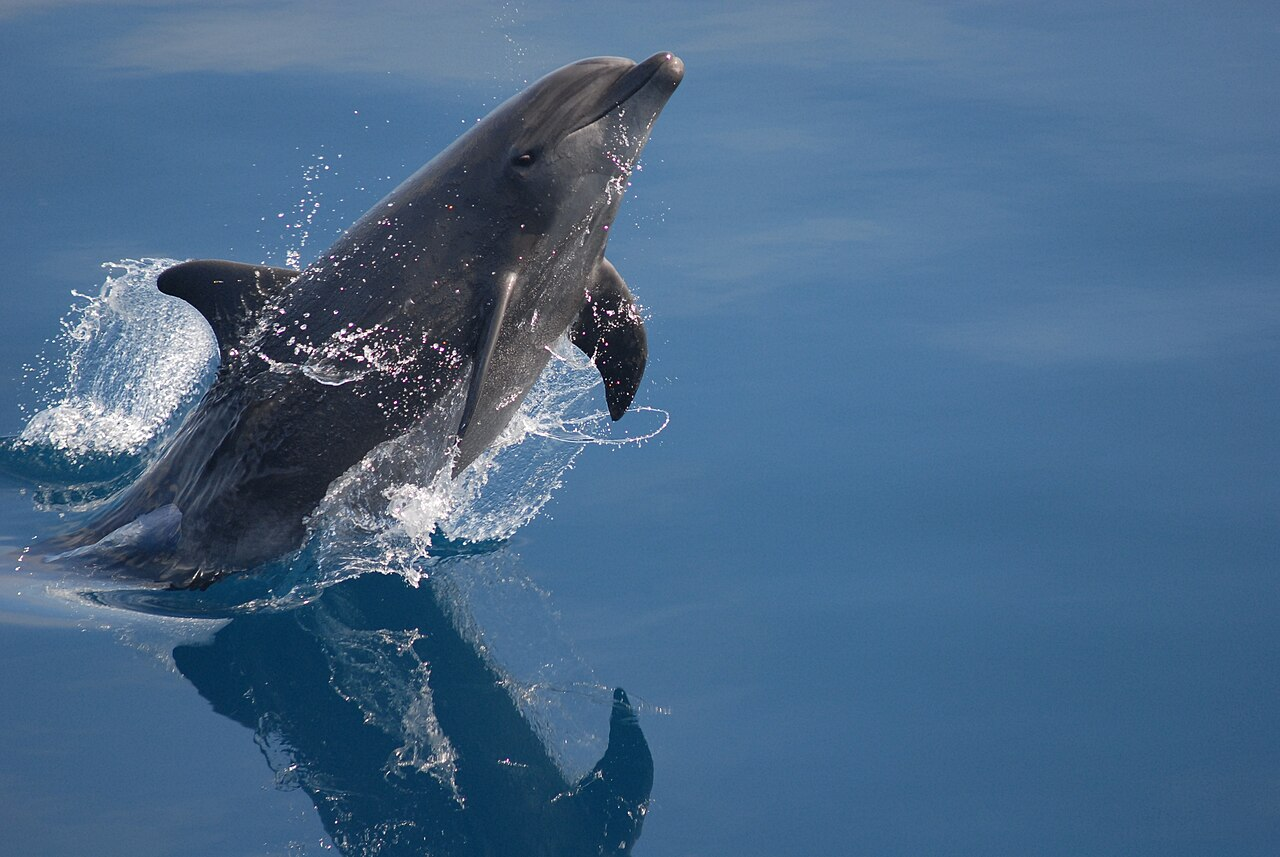
\includegraphics[width=\linewidth]{dolphins.jpg}\par\smallskip
      {\small \textbf{Դելֆինները} քնում են ուղեղի \textbf{կեսով}, որ չխեղդվեն։ Քունն ավելի կարևոր է, քան «չխեղդվելը»։}
    \end{column}
    \begin{column}{0.3\textwidth}
      \onslide<2->{%
      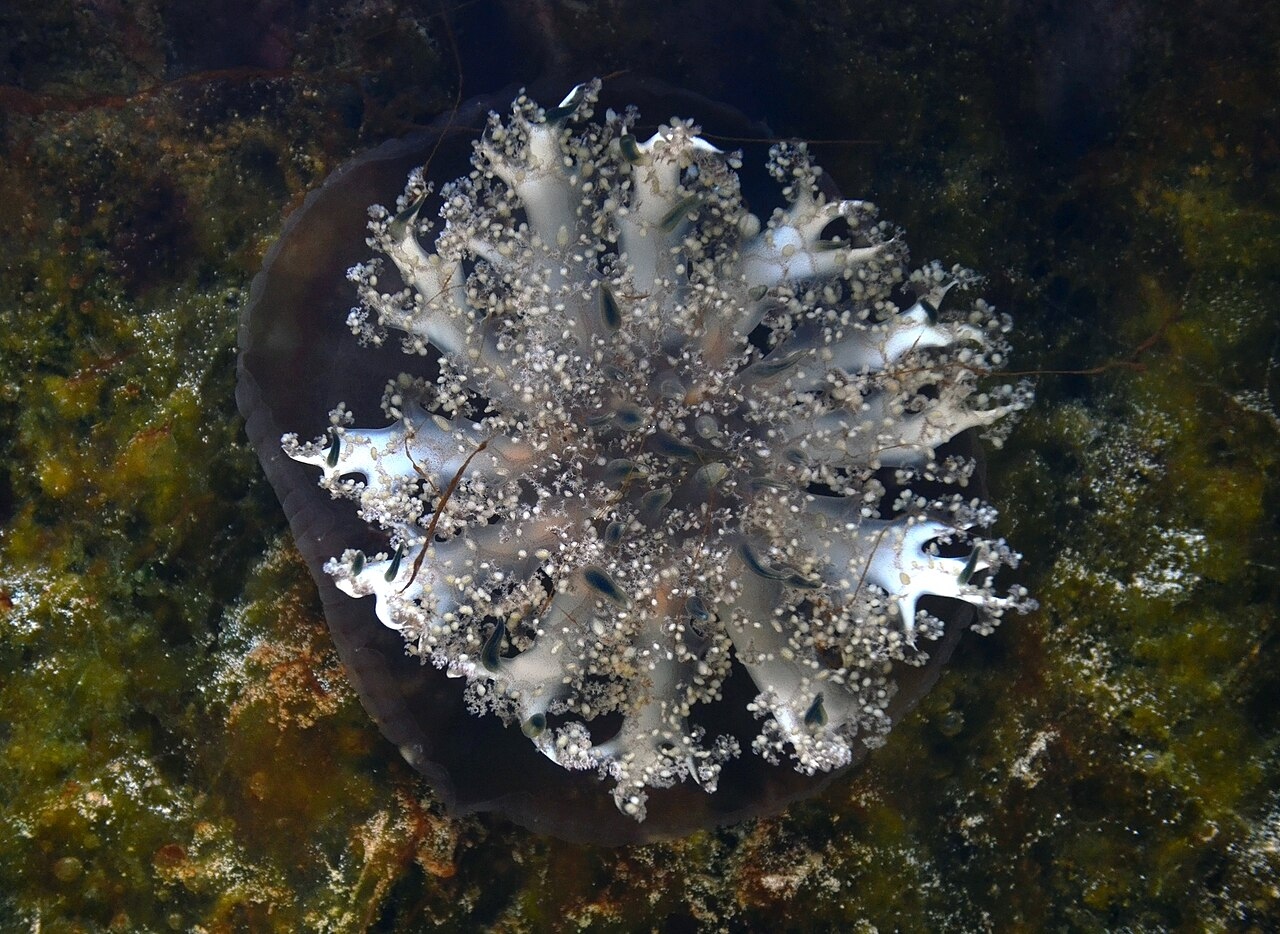
\includegraphics[width=\linewidth]{jellyfish.jpg}\par\smallskip
      {\small Բըրնեթը (2016)՝ «Մեդուզաները չեն քնում, բայց նրանք ուղեղ էլ չունեն»։}}
    \end{column}
    \begin{column}{0.33\textwidth}
      \onslide<3->{%
      \begin{scienceupdate}
        2017-ին պարզվեց, որ \textbf{Cassiopea} մեդուզան (նկարում) քնի նման վիճակ ունի. գիշերը դանդաղում է, դժվար է «արթնանում», իսկ եթե չթողնես հանգստանա, հաջորդ օրը ավելի պասիվ է։ \textbf{Առանց ուղեղի}։
      \end{scienceupdate}}
    \end{column}
  \end{columns}
  \source{Nath et al., Current Biology, 2017}
\end{frame}

\begin{frame}{Ինչի՞ համար է քունը. վարկածներ}
  \tcbset{hyp/.style={fontupper=\footnotesize, top=0.8mm, bottom=0.8mm}}
  \begin{columns}[T]
    \begin{column}{0.31\textwidth}
      \begin{card}[hyp, colback=mint!30!cardwhite]\emoji{rat}\ \textbf{Վերականգնում}. առանց քնի առնետների վերքերը դանդաղ են լավանում\end{card}
      \begin{card}[hyp, colback=mint!30!cardwhite]\emoji{tiger}\ \textbf{Թաքնվել} գիշերային գիշատիչներից\end{card}
    \end{column}
    \begin{column}{0.31\textwidth}
      \begin{card}[hyp, colback=lavender!35!cardwhite]\emoji{construction}\ \textbf{«Էտում»}. թույլ կապերը թուլանում են (synaptic pruning)\end{card}
      \begin{card}[hyp, colback=lavender!35!cardwhite]\emoji{puzzle}\ \textbf{Հիշողություն}. օրվա հիշողությունները դասավորվում են\end{card}
    \end{column}
    \begin{column}{0.31\textwidth}
      \begin{card}[hyp, colback=peach!35!cardwhite]\emoji{thought}\ \textbf{Զգացմունքներ}. բացասականը մեղմանում է\end{card}
      \begin{card}[hyp, colback=peach!35!cardwhite]\emoji{broom}\ \textbf{Աղբահանություն}. ուղեղը մաքրում է թափոնները\end{card}
    \end{column}
  \end{columns}
  \begin{chatbox}
    Քո վարկածը՞։ Ինչի՞ համար ես \textbf{դու} քնում (կատակով էլ կարելի է)
  \end{chatbox}
\end{frame}

\begin{frame}{Քունը պարզապես հանգիստ չէ}
  \begin{columns}[T]
    \begin{column}{0.31\textwidth}
      \begin{card}
        \centering\bigemoji[0.8cm]{muscle}\ \bigemoji[0.8cm]{tv}\par\smallskip
        Աղյուս ես կրել, թե ամբողջ օրը մուլտ նայել, \textbf{նույնքան} ես քնում
      \end{card}
    \end{column}
    \begin{column}{0.31\textwidth}
      \onslide<2->{%
      \begin{card}
        \centering\bigemoji[0.8cm]{car}\par\smallskip
        Քնած մարմնի մետաբոլիզմը իջնում է ընդամենը \textbf{5-10\%}-ով. ինչպես ծխացող շարժիչով 80-ից 72 կմ/ժ դանդաղելը
      \end{card}}
    \end{column}
    \begin{column}{0.31\textwidth}
      \onslide<3->{%
      \begin{card}
        \centering\bigemoji[0.8cm]{chipmunk}\par\smallskip
        Ձմեռային քուն մտած սկյուռները ժամանակ առ ժամանակ \textbf{արթնանում են, որ քնեն}
      \end{card}}
    \end{column}
  \end{columns}
  \vspace{2mm}
  \onslide<4->{\centering Ու մարաթոնի ընթացքում մարդիկ հազվադեպ են քնում. քնի ժամը որոշում է ոչ թե հոգնածությունը, այլ \textbf{ներքին ժամացույցը}։\par}
\end{frame}

\begin{frame}{Ներքին ժամացույց (circadian rhythm)}
  \centering
  % Schematic 24-hour body clock: melatonin (low all day, rises after dark,
% peaks around 3 a.m.) and core body temperature (peaks late afternoon,
% lowest around 4-5 a.m.). Shapes follow the textbook curves; the y axis is
% deliberately unitless ("schematic").
\begin{tikzpicture}
  \begin{axis}[
      width=13.6cm, height=5.0cm,
      xmin=6, xmax=30, ymin=0, ymax=1.15,
      xtick={6,9,12,15,18,21,24,27,30},
      xticklabels={06:00, 09:00, 12:00, 15:00, 18:00, 21:00, 00:00, 03:00, 06:00},
      ytick=\empty, axis y line=none, axis x line*=bottom,
      tick label style={font=\small, text=plum}, axis line style={plum},
      clip=false,
    ]
    % night shading
    \fill[lavender!60] (axis cs:22,0) rectangle (axis cs:30,1.15);
    \node[font=\blackfont\small, text=lavenderdark] at (axis cs:26,1.07) {\emoji{moon}\ գիշեր};
    \node[font=\blackfont\small, text=peachdark] at (axis cs:8.6,1.07) {\emoji{sun}\ ցերեկային լույս};

    % melatonin
    \addplot[name path=mel, domain=6:30, samples=160, line width=2.2pt, amBlue]
      {0.04 + 0.86*exp(-((x-27)^2)/(2*2.3^2))};
    \path[name path=base] (axis cs:6,0) -- (axis cs:30,0);
    \addplot[amBlue!15] fill between[of=mel and base];

    % body temperature
    \addplot[domain=6:30, samples=160, line width=2.2pt, amRed, dashed]
      {0.55 + 0.27*cos(15*(x-17))};

    % labels
    \node[anchor=west, font=\small, text=amBlue, align=left]
      at (axis cs:6.3,0.2) {\textbf{Մելատոնին} («քնի հորմոն»)՝\\ ցածր է, քանի դեռ լույս է ընկնում աչքերիդ};
    \node[anchor=north, font=\small, text=amRed]
      at (axis cs:17,0.76) {\textbf{Մարմնի ջերմաստիճան} (36-37 °C)};
    \draw[plum!60, line width=1pt, densely dotted] (axis cs:23,0) -- (axis cs:23,0.98)
      node[anchor=south, font=\small, text=plum, fill=lavender!60, inner sep=1pt] {քուն};
  \end{axis}
\end{tikzpicture}
\par\smallskip
  \begin{columns}[T]
    \begin{column}{0.47\textwidth}
      \small Էպիֆիզը (pineal gland) արտադրում է \textbf{մելատոնին}. շատ լույս՝ քիչ մելատոնին։\\
      Մարմինն ամենացուրտն է վաղ առավոտյան։
    \end{column}
    \begin{column}{0.47\textwidth}
      \small\emoji{airplane}\ Ջեթ-լեգ՝ լույսը նոր ժամային գոտու է, ուղեղը՝ հնի։\\ \emoji{phone}\ Արհեստական լույսն էլ է շեղում ժամացույցը։
    \end{column}
  \end{columns}
\end{frame}

\begin{frame}{Մեկ գիշերը՝ փուլերով}
  \centering
  % A typical night (hypnogram): ~90-minute cycles, deep sleep (N3) mostly in
% the first half, REM periods getting longer towards morning. Illustrative
% data for a healthy young sleeper, not one real recording.
\begin{tikzpicture}
  \begin{axis}[
      width=13.8cm, height=5.3cm,
      xmin=0, xmax=8, ymin=-0.4, ymax=5.0,
      xtick={0,1,...,8},
      xticklabels={23:00, 00:00, 01:00, 02:00, 03:00, 04:00, 05:00, 06:00, 07:00},
      ytick={0,1,2,3,4},
      yticklabels={\textbf{Խորը (N3)}, N2, N1, \textcolor{amRed}{\textbf{REM}}, Արթուն},
      tick label style={font=\small, text=plum}, axis line style={plum},
      axis x line*=bottom, axis y line*=left,
      ymajorgrids, grid style={plum!10},
      clip=false,
    ]
    \fill[amBlue!10] (axis cs:0,-0.4) rectangle (axis cs:8,0.4);
    \fill[amRed!8]   (axis cs:0,2.6) rectangle (axis cs:8,3.4);

    \addplot[const plot, line width=1.6pt, plum] coordinates {
      (0,4) (0.12,2) (0.25,1) (0.45,0) (1.05,1) (1.25,3) (1.4,1) (1.6,0)
      (2.3,1) (2.75,3) (3.05,1) (3.3,0) (3.6,1) (4.2,3) (4.6,2) (4.65,4)
      (4.72,1) (5.45,3) (6.0,1) (6.6,3) (7.3,2) (7.4,1) (7.6,3) (7.95,4) (8,4)};

    % REM periods in red on top
    \foreach \a/\b in {1.25/1.4, 2.75/3.05, 4.2/4.6, 5.45/6.0, 6.6/7.3, 7.6/7.95}{
      \edef\temp{\noexpand\draw[amRed, line width=4pt] (axis cs:\a,3) -- (axis cs:\b,3);}
      \temp
    }

    % one cycle brace, above the curve
    \draw[decorate, decoration={brace, amplitude=5pt}, line width=1pt, plum!70]
      (axis cs:0.05,4.25) -- (axis cs:1.42,4.25)
      node[midway, above=5pt, font=\small, text=plum] {1 ցիկլ՝ մոտ 90 րոպե};

    \node[visible on=<2->, font=\blackfont\small, text=amBlue, fill=cream, inner sep=2pt, anchor=west]
      (deep) at (axis cs:4.75,0.45) {խորը քունը՝ գիշերվա սկզբում};
    \draw[visible on=<2->, -{Stealth}, amBlue, line width=1pt] (deep.west) to[out=180, in=40] (axis cs:3.3,0.1);
    \node[visible on=<3->, font=\blackfont\small, text=amRed, fill=cream, inner sep=2pt]
      (rem) at (axis cs:4.6,4.6) {REM-ը (երազները) երկարում է դեպի առավոտ};
    \draw[visible on=<3->, -{Stealth}, amRed, line width=1pt] (rem.east) to[out=0, in=100] (axis cs:6.9,3.25);
  \end{axis}
\end{tikzpicture}
\par\medskip
  {\small N1-ից N3 ուղեղի ակտիվությունը թուլանում է, ու ավելի դժվար է արթնանալ։ \textbf{REM}-ի (rapid eye movement) ժամանակ ուղեղը նույնքան ակտիվ է, որքան արթուն ժամանակ, ու հենց այդ ժամանակ ենք երազ տեսնում։}
\end{frame}

\begin{frame}{Երազի ժամանակ մարմինն անջատված է}
  \begin{columns}[T]
    \begin{column}{0.31\textwidth}
      \begin{card}[colback=mint!30!cardwhite]
        \centering\mascot[1.3cm]{sleepy}\par
        {\blackfont Նորմալ REM}\par\smallskip
        \raggedright Երազում վազում ես, բայց շարժումների «անջատիչը» \textbf{անջատված} է (REM atonia)։ Այլապես կխաղայինք մեր երազները
      \end{card}
    \end{column}
    \begin{column}{0.31\textwidth}
      \onslide<2->{%
      \begin{card}[colback=lavender!35!cardwhite]
        \centering\mascot[1.3cm]{scared}\par
        {\blackfont Քնի կաթված}\par\smallskip
        \raggedright Արթնացար, բայց անջատիչը \textbf{դեռ անջատված է}։ Չես կարողանում շարժվել (sleep paralysis)
      \end{card}}
    \end{column}
    \begin{column}{0.31\textwidth}
      \onslide<3->{%
      \begin{card}[colback=peach!35!cardwhite]
        \centering\mascot[1.3cm]{confused}\par
        {\blackfont Լուսնոտություն}\par\smallskip
        \raggedright Անջատիչը \textbf{բավարար չի աշխատում}։ Ավելի հաճախ է երեխաների մոտ ու հաճախ ընտանեկան է
      \end{card}}
    \end{column}
  \end{columns}
\end{frame}

\begin{frame}{«Ընկնում եմ». հիպնիկ ցնցում}
  \begin{columns}[c]
    \begin{column}{0.5\textwidth}
      \begin{poll}
        Բարձրացրու ձեռքդ, եթե քնելիս երբևէ \textbf{հանկարծ ցնցվել ես}, կարծես ինչ-որ տեղից ընկնում ես (hypnic jerk)։
      \end{poll}
      \vspace{2mm}
      \onslide<2->{\small Երեխաների մոտ ավելի հաճախ է, տարիքի հետ պակասում է, բայց չի անհետանում։ \textbf{Անվնաս է}։}
    \end{column}
    \begin{column}{0.44\textwidth}
      \onslide<3->{%
      {\blackfont Վարկածներ}\par\smallskip
      \begin{itemize}
        \item Ուղեղը քնելը շփոթում է «մեռնելու» հետ ու փորձում է արթնացնել։ Համոզիչ չէ
        \item<4-> Ժառանգություն այն ժամանակներից, երբ \textbf{ծառերի վրա} էինք քնում \emoji{monkey}\emoji{tree}. թեքվել նշանակում էր ընկնել
        \item<5-> Կամ միանգամայն այլ բան։ Իրականում \textbf{չգիտենք}
      \end{itemize}}
    \end{column}
  \end{columns}
\end{frame}

\begin{frame}{Քնի կաթված. մղձավանջ աչքերը բաց}
  \begin{columns}[c]
    \begin{column}{0.46\textwidth}
      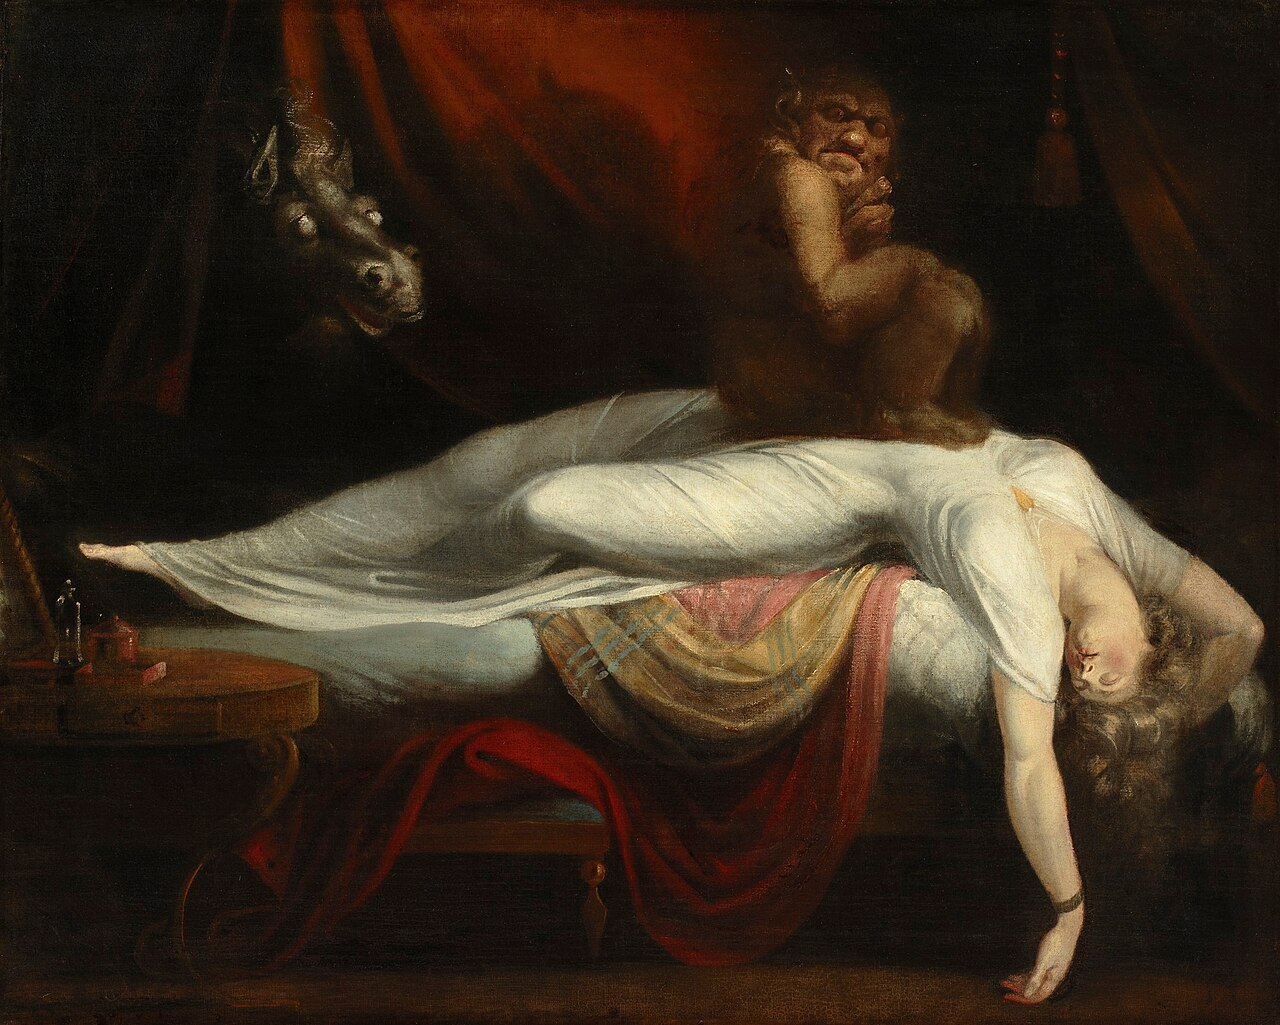
\includegraphics[width=\linewidth]{nightmare_fuseli.jpg}\par
      {\scriptsize Հենրի Ֆյուզելի, «Մղձավանջ», 1781}
    \end{column}
    \begin{column}{0.48\textwidth}
      \begin{itemize}
        \item Ուղեղը «մոռանում է» շարժումները նորից միացնել
        \item<2-> Անօգնականությունը միացնում է \textbf{վախը}, իսկ վախը կարող է հալյուցինացիաներ առաջացնել
        \item<3-> Սենյակում «ինչ-որ մեկի» ներկայություն, կրծքին նստած դև (սուկուբի լեգենդը), այլմոլորակայինների առևանգում \emoji{alien}
        \item<4-> Սովորաբար տևում է կարճ ու \textbf{վտանգավոր չէ}
      \end{itemize}
    \end{column}
  \end{columns}
\end{frame}

\begin{frame}{Որքա՞ն հաճախ է պատահում քնի կաթվածը}
  \begin{columns}[c]
    \begin{column}{0.56\textwidth}
      \centering
      % Lifetime prevalence of sleep paralysis (at least one episode).
% Sharpless & Barber, Sleep Medicine Reviews 2011: 35 studies, 36,533 people.
\begin{tikzpicture}
  \begin{axis}[
      width=7.0cm, height=5.4cm,
      ybar, bar width=1.05cm, bar shift=0pt,
      ymin=0, ymax=40,
      symbolic x coords={general, students, treatment},
      xtick=data,
      xticklabels={{Բոլորը}, {Ուսանողներ}, {Հոգեբուժական\\ պացիենտներ}},
      xticklabel style={align=center, font=\small, text width=2.3cm},
      ytick={0,10,20,30,40}, yticklabel={\pgfmathprintnumber{\tick}\%},
      tick label style={font=\small, text=plum}, axis line style={plum},
      axis x line*=bottom, axis y line*=left, ymajorgrids, grid style={plum!10},
      nodes near coords={\pgfmathprintnumber[fixed, precision=1]{\pgfplotspointmeta}\%},
      nodes near coords style={font=\blackfont\small, text=plum},
      enlarge x limits=0.25,
    ]
    \addplot[fill=amBlue, draw=none] coordinates {(general,7.6)};
    \addplot[fill=amOrange, draw=none] coordinates {(students,28.3)};
    \addplot[fill=amBlue, draw=none] coordinates {(treatment,31.9)};
  \end{axis}
\end{tikzpicture}
\par
      {\scriptsize Գոնե մեկ անգամ կյանքում. 35 հետազոտություն, 36\,533 մարդ}
    \end{column}
    \begin{column}{0.4\textwidth}
      \begin{card}[colback=butter!45!cream]
        Ուսանողների \textbf{մոտ 28\%}-ը գոնե մեկ անգամ ունեցել է։ Այսինքն՝ այս Zoom-ում հավանաբար ամեն չորրորդը։ Կապված է քնի պակասի ու անկանոն ռեժիմի հետ։
      \end{card}
      \vspace{2mm}
      \onslide<2->{%
      \begin{card}[colback=mint!30!cardwhite]
        Եթե պատահի՝ հիշիր, որ դա ուղեղի «բագ» է, ոչ թե դև։ Մի քանի վայրկյանից անցնում է։
      \end{card}}
    \end{column}
  \end{columns}
  \source{Sharpless \& Barber, Sleep Medicine Reviews, 2011}
\end{frame}

\begin{frame}{Ինչու են երազներն այդքան տարօրինակ}
  \begin{columns}[c]
    \begin{column}{0.58\textwidth}
      \begin{itemize}
        \item REM-ի ժամանակ ուղեղը \textbf{դասավորում է հիշողությունները}՝ հները կապում է նորերի հետ
        \item Ինչպես ճանապարհի վերանորոգումը, որ արվում է, երբ մեքենաներ չկան. քնած ժամանակ դրսից տեղեկություն չի գալիս
        \item<2-> Հիշողությունները «վերապրվում» են խառը հերթականությամբ, դրա համար էլ երազը անհեթեթ է
        \item<3-> Ճակատային բլթերը փորձում են այդ խառնաշփոթից պատմություն սարքել, ու երազում ամեն ինչ իրական է թվում
      \end{itemize}
    \end{column}
    \begin{column}{0.36\textwidth}
      \centering
      \bigemoji[1.8cm]{construction}
    \end{column}
  \end{columns}
\end{frame}

\begin{frame}{Կրկնվող երազներ ու քնկոտ նորածիններ}
  \begin{columns}[T]
    \begin{column}{0.47\textwidth}
      \begin{card}[colback=peach!35!cardwhite]
        \emoji[1.3em]{fire}\ {\blackfont Կրկնվող երազներ}\par\smallskip
        Ինչն անհանգստացնում է, դրա մասին շատ ես մտածում, շատ նոր հիշողություններ ես ունենում, ու դրանք հաճախ են հայտնվում երազում։\par\smallskip
        Բըրնեթը գիրքը գրելիս երազում \textbf{այրում էր իր հրատարակչի գրասենյակը}։
      \end{card}
    \end{column}
    \begin{column}{0.47\textwidth}
      \onslide<2->{%
      \begin{card}[colback=lavender!35!cardwhite]
        \emoji[1.3em]{baby}\ {\blackfont Նորածիններ}\par\smallskip
        Քնում են օրվա կեսից ավելին, ու նրանց քնի մոտ կեսը REM է (մեծահասակների մոտ՝ մոտ 20\%)։ Գուցե այդպես է ուղեղը «կառուցվում»։
      \end{card}}
    \end{column}
  \end{columns}
\end{frame}

\begin{frame}{Առանց քնի}
  \begin{columns}[c]
    \begin{column}{0.48\textwidth}
      \begin{itemize}
        \item Ուշադրությունն ու խնդիրներ լուծելը վատանում են, սթրեսն ու ջղայնությունը աճում են
        \item Ուղեղը սկսում է «միկրոքներ»՝ մի քանի վայրկյանով
        \item Չեռնոբիլի ու Challenger-ի աղետները կապում են հոգնած անձնակազմի հետ
        \item Երկար ժամանակ քիչ քնելը վնասում է իմունիտետը, սիրտը ու քաշը
      \end{itemize}
    \end{column}
    \begin{column}{0.48\textwidth}
      \centering
      \onslide<2->{%
      \begin{meme}[6.8cm]{this_is_fine.jpg}
        \memecap{0.5}{1.12}{Քննաշրջան, 4 ժամ քուն}
        \memecap[minimum width=3.4cm, minimum height=1.1cm]{0.785}{0.83}{Ամեն ինչ\\ նորմալ է}
      \end{meme}}
    \end{column}
  \end{columns}
\end{frame}

\begin{frame}{Քանի՞ ժամ է պետք}
  \begin{columns}[c]
    \begin{column}{0.6\textwidth}
      % Recommended sleep per day by age: National Sleep Foundation panel
% (Hirshkowitz et al., Sleep Health, 2015). Bars show the recommended
% RANGE (floating bars), labelled with the range. Teens highlighted.
\begin{tikzpicture}
  \begin{axis}[
      width=8.2cm, height=5.8cm,
      xmin=0, xmax=20.5, ymin=-0.6, ymax=5.6, y dir=reverse,
      ytick={0,1,2,3,4,5},
      yticklabels={Նորածին, 1-2 տարեկան, 6-13 տարեկան, \textbf{14-17 տարեկան}, 26-64 տարեկան, 65+ տարեկան},
      xtick={0,4,8,12,16}, xlabel={քնի ժամեր օրական}, xlabel style={font=\small, text=plum},
      tick label style={font=\small, text=plum}, axis line style={plum},
      axis x line*=bottom, axis y line*=left, xmajorgrids, grid style={plum!10},
      clip=false,
    ]
    \foreach \y/\lo/\hi/\c in {0/14/17/amBlue, 1/11/14/amBlue, 2/9/11/amBlue, 3/8/10/amOrange, 4/7/9/amBlue, 5/7/8/amBlue}{
      \edef\temp{\noexpand\fill[\c, rounded corners=1.5pt] (axis cs:\lo,\y-0.32) rectangle (axis cs:\hi,\y+0.32);
                 \noexpand\node[anchor=west, font=\noexpand\blackfont\noexpand\small, text=plum] at (axis cs:\hi,\y) {\lo-\hi\noexpand\,ժ};}
      \temp
    }
  \end{axis}
\end{tikzpicture}

    \end{column}
    \begin{column}{0.36\textwidth}
      \begin{chatbox}
        Քանի՞ ժամ քնեցիր երեկ գիշեր։ Գրիր միայն թիվը։
      \end{chatbox}
      \vspace{3mm}
      \onslide<2->{%
      \begin{bookquote}
        Եթե այս գիրքը կարդալիս քունդ տանի, դա ձանձրալի չէ, դա \textbf{բուժիչ} է։
      \end{bookquote}}
    \end{column}
  \end{columns}
  \source{Hirshkowitz et al., Sleep Health, 2015}
\end{frame}

% ---------------------------------------------------------------- fear
\topicopener{scream}{Վախ}{Կամ հին խալաթ է, կամ արյունարբու մարդասպան}{«Կռվիր կամ փախիր» ռեակցիան}{scared}

\begin{frame}{Մութ սենյակ, դռան մոտ՝ ինչ-որ մեկը}
  \centering
  % Same door, same dressing gown: lights off (panel 1) vs lights on (panel 2,
% revealed on slide 2).
\begin{tikzpicture}[
    paneltitle/.style={font=\blackfont\normalsize, text=#1, anchor=north west},
  ]
  % robe outline as a reusable path (hood, shoulders, sleeves, body)
  \def\robe{
    (-0.5,0.95) .. controls (-0.62,1.85) and (0.62,1.85) .. (0.5,0.95)
    -- (1.0,0.7) -- (1.25,-0.75) -- (0.9,-0.8) -- (0.78,0.15)
    -- (0.98,-2.25) -- (-0.98,-2.25) -- (-0.78,0.15)
    -- (-0.9,-0.8) -- (-1.25,-0.75) -- (-1.0,0.7) -- cycle}

  % ================= panel 1: lights off ===============================
  \begin{scope}[shift={(-3.6,0)}]
    \fill[night, rounded corners=4mm] (-3.3,-2.7) rectangle (3.3,2.9);
    \fill[night!70!black] (-1.7,-2.7) rectangle (1.7,2.1);                % door
    \draw[night!40, line width=0.6pt] (-1.4,0.4) rectangle (1.4,1.85) (-1.4,-2.45) rectangle (1.4,0.1);
    \fill[night!40] (1.35,-0.1) circle (0.09);                               % knob
    \fill[black!85] (0,1.8) circle (0.08);                                   % hook
    \fill[black, opacity=0.95] \robe;
    \fill[black] (0,1.12) ellipse (0.3 and 0.36);
    \fill[amRed!80!amOrange] (-0.11,1.15) ellipse (0.07 and 0.04) (0.11,1.15) ellipse (0.07 and 0.04);
    \draw[black, line width=3pt, line cap=round] (0.95,-0.45) -- (1.65,1.05);  % "axe" (the belt end)
    \fill[black] (1.42,0.7) -- (2.05,1.25) .. controls (2.1,0.9) and (2.0,0.65) .. (1.82,0.32) -- cycle;
    \node[paneltitle=white] at (-3.15,2.8) {\emoji{moon}\ Գիշերվա 2-ը, մութ};
    \pic[scale=0.5] at (-2.4,-1.95) {noggin=scared};
    \node[say, callout absolute pointer={(-2.35,-1.35)}, font=\handfont\small, inner sep=3pt]
      at (-2.2,-0.3) {ԿԱՑՆՈՎ\\ ՄԱՐԴԱՍՊԱՆ};
  \end{scope}

  % ================= panel 2: lights on ================================
  \begin{scope}[shift={(3.6,0)}, visible on=<2->]
    \fill[butter!60!cream, rounded corners=4mm] (-3.3,-2.7) rectangle (3.3,2.9);
    \fill[peach] (-1.7,-2.7) rectangle (1.7,2.1);
    \draw[peachdark!60, line width=0.6pt] (-1.4,0.4) rectangle (1.4,1.85) (-1.4,-2.45) rectangle (1.4,0.1);
    \fill[peachdark] (1.35,-0.1) circle (0.09);
    \fill[plum!70] (0,1.8) circle (0.08);
    \filldraw[fill=lavender, draw=lavenderdark, line width=1pt] \robe;
    \fill[lavender!70!white] (0,1.12) ellipse (0.3 and 0.36);
    \draw[lavenderdark, line width=3pt, line cap=round] (-0.8,-0.35) -- (0.8,-0.35);
    \draw[lavenderdark, line width=3pt, line cap=round] (0.3,-0.35) -- (0.45,-1.25);
    \draw[lavenderdark, line width=3pt, line cap=round] (0.45,-0.35) -- (0.95,-1.05);
    \foreach \p in {(-0.4,0.3),(0.3,0.6),(-0.5,-1.5),(0.5,-1.8),(0.0,-0.9),(-0.15,0.7)}
      \fill[white, opacity=0.6] \p circle (0.05);
    \node[paneltitle=plum] at (-3.15,2.8) {\emoji{bulb}\ Լույսը վառեցինք};
    \pic[scale=0.5] at (-2.4,-1.95) {noggin=smug};
    \node[say, callout absolute pointer={(-2.35,-1.35)}, font=\handfont\small, inner sep=3pt]
      at (-2.2,-0.3) {...Ես գիտեի։};
    \node[font=\blackfont\small, text=lavenderdark, fill=cardwhite, rounded corners=2pt, inner sep=3pt]
      at (1.55,-2.4) {\emoji{check}\ ընդամենը խալաթ է};
  \end{scope}
\end{tikzpicture}

\end{frame}

\begin{frame}{Ավելի լավ է ապահով, քան ափսոս}
  \begin{columns}[T]
    \begin{column}{0.47\textwidth}
      \begin{card}[colback=mint!30!cardwhite]
        \emoji[1.5em]{runner}\ {\blackfont Նախնի 1}\par\smallskip
        Թփի մեջ ինչ-որ բան շարժվեց, \textbf{փախավ}։ Կենդանի մնաց ու երեխաներ ունեցավ
      \end{card}
    \end{column}
    \begin{column}{0.47\textwidth}
      \onslide<2->{%
      \begin{card}[colback=brainpink!30!cardwhite]
        \emoji[1.5em]{tiger}\ {\blackfont Նախնի 2}\par\smallskip
        «Սպասենք, համոզվենք, որ իսկապես վագր է»։ Դարձավ վագրի նախաճաշը
      \end{card}}
    \end{column}
  \end{columns}
  \vspace{1mm}
  \onslide<3->{%
  \begin{bookquote}
    Ուղեղի համար առօրյան լարախաղացություն է կատաղի մեղրագայլերով ու կոտրված ապակիներով լի փոսի վրայով։
  \end{bookquote}}
  \onslide<4->{\centering Մենք \textbf{առաջինի} ժառանգներն ենք. վախը կրակում է նախ, մտածում՝ հետո։\par}
\end{frame}

\begin{frame}{Վախի երկու ճանապարհ}
  \centering
  % Fear pathways: senses -> thalamus ("main station") -> amygdala (fast,
% rough alarm) -> hypothalamus ("taxi rank") -> body; and the slow, careful
% route through the cortex that only later says "it was a balloon".
\begin{tikzpicture}[
    part/.style={draw=#1, line width=1.2pt, fill=#1!10!cardwhite, rounded corners=3mm,
                 align=center, inner sep=5pt, text width=2.6cm, font=\small, text=plum},
    road/.style={-{Stealth[length=3.2mm]}, line width=2pt, #1},
  ]
  \path[use as bounding box] (-7.2,-2.75) rectangle (7.2,2.75);

  \node[part=plum] (sense) at (-5.85,0)
    {\bigemoji[0.7cm]{eye}\,\bigemoji[0.7cm]{ear}\\[2pt] \textbf{Զգայարաններ}\\ «ԲՈՒ՛Մ»};
  \node[part=plum] (thal) at (-2.6,0)
    {\bigemoji[0.7cm]{station}\\[2pt] \textbf{Թալամուս}\\ գլխավոր կայարանը};
  \draw[road=plum] (sense) -- (thal);

  % fast road
  \node[part=amRed, visible on=<2->] (amy) at (0.9,1.55)
    {\bigemoji[0.7cm]{bell}\\[2pt] \textbf{Նշաձև մարմին}\\ ահազանգը};
  \node[part=amRed, visible on=<2->] (hypo) at (4.3,1.55)
    {\bigemoji[0.7cm]{taxi}\\[2pt] \textbf{Հիպոթալամուս}\\ տաքսիների կանգառը};
  \node[part=amRed, visible on=<2->, text width=1.75cm] (body) at (6.3,-0.45)
    {\bigemoji[0.7cm]{anatomicalheart}\\[2pt] \textbf{Մարմին}\\ մարտական\\ վիճակ};
  \draw[road=amRed, visible on=<2->] (thal.north east) to[out=40, in=180]
    node[pos=0.45, above left=-1pt, font=\blackfont\small, text=amRed] {ԱՐԱԳ ճամփա} (amy.west);
  \draw[road=amRed, visible on=<2->] (amy) -- (hypo);
  \draw[road=amRed, visible on=<2->] (hypo.south east) to[out=-30, in=90] (body.north);

  % slow road
  \node[part=amBlue, visible on=<3->] (cortex) at (0.9,-1.65)
    {\bigemoji[0.7cm]{detective}\\[2pt] \textbf{Կեղև}\\ խուզարկուն};
  \draw[road={amBlue, dashed}, visible on=<3->] (thal.south east) to[out=-40, in=180]
    node[pos=0.45, below left=-1pt, font=\blackfont\small, text=amBlue] {դանդաղ ճամփա} (cortex.west);
  \node[say, visible on=<3->, callout absolute pointer={(cortex.east)}, text width=2.6cm, font=\handfont\normalsize]
    at (3.75,-1.85) {Փուչիկ էր ընդամենը։ Հանգստացե՛ք... ուշ է՞};
\end{tikzpicture}

\end{frame}

\begin{frame}{Նշաձև մարմինն ընդդեմ կեղևի}
  \begin{columns}[c]
    \begin{column}{0.58\textwidth}
      \centering
      \begin{meme}[7.6cm]{woman_yelling_at_cat.jpg}
        \memecap{0.25}{0.91}{նշաձև մարմին (amygdala)}
        \memecap{0.75}{0.91}{կեղև (cortex)}
        \memecap{0.2}{0.18}{ԿԱՑՆՈՎ\\ ՄԱՐԴԱՍՊԱՆ}
        \memecap{0.76}{0.18}{դա խալաթ է}
      \end{meme}
    \end{column}
    \begin{column}{0.38\textwidth}
      \onslide<2->{%
      \begin{card}[colback=brainpink!25!cardwhite]
        Նշաձև մարմինը նրբություններ չի հասկանում։ Փուչիկը պայթում է, ու վախը գալիս է \textbf{նախքան} կեղևը կհասցնի ասել, որ վտանգ չկա։
      \end{card}}
    \end{column}
  \end{columns}
\end{frame}

\begin{frame}{Նյարդային համակարգը՝ սիթքոմ}
  \centering
  \begin{tikzpicture}[edge/.style={plum, line width=1pt}]
    \node[flow=4.4cm, fill=butter!50!cardwhite] (all) at (-1,2.9) {\textbf{Նյարդային համակարգ}};
    \node[flow] (cns) at (-4.6,1.6) {\textbf{Կենտրոնական}\\ ուղեղ ու ողնուղեղ};
    \node[flow] (pns) at (1.4,1.6) {\textbf{Ծայրամասային}\\ մնացած նյարդերը};
    \node[flow, visible on=<2->] (som) at (-1.6,0.2) {\textbf{Սոմատիկ}\\ կամային շարժումներ};
    \node[flow, visible on=<2->] (aut) at (3.6,0.2) {\textbf{Վեգետատիվ}\\ ինքնաշխատ, օրգաններ};
    \node[flow=3.6cm, fill=brainpink!40!cardwhite, visible on=<4->] (sym) at (1.3,-2.1)
      {\emoji{scream}\ \textbf{Սիմպաթիկ}\\ պարանոյիկ հարևանը. «Կռվի՛ր կամ փախի՛ր»};
    \node[flow=3.6cm, fill=mint!40!cardwhite, visible on=<3->] (para) at (5.3,-2.1)
      {\emoji{couch}\ \textbf{Պարասիմպաթիկ}\\ բազմոցի տղան. «Հանգստացի՛ր»};
    \draw[edge] (all) -- (cns); \draw[edge] (all) -- (pns);
    \draw[edge, visible on=<2->] (pns) -- (som); \draw[edge, visible on=<2->] (pns) -- (aut);
    \draw[edge, visible on=<3->] (aut) -- (para);
    \draw[edge, visible on=<4->] (aut) -- (sym);
  \end{tikzpicture}
\end{frame}

\begin{frame}{Մարմինը՝ մարտական պատրաստության}
  \setbeamertemplate{itemize item}{}
  \begin{columns}[T]
    \begin{column}{0.47\textwidth}
      \begin{card}
        \begin{itemize}
          \item \emoji[1.2em]{eyes}\ Բիբերը լայնանում են. ավելի շատ լույս, որ վտանգը տեսնես
          \item \emoji[1.2em]{anatomicalheart}\ Սիրտն արագ է խփում, արյունը գնում է մկաններ
          \item \emoji[1.2em]{lungs}\ Արագ շնչառություն՝ ավելի շատ թթվածին
          \item \emoji[1.2em]{muscle}\ Մկանները լարվում են՝ պատրաստ վազելու կամ կռվելու
        \end{itemize}
      \end{card}
    \end{column}
    \begin{column}{0.47\textwidth}
      \onslide<2->{%
      \begin{card}
        \begin{itemize}
          \item \emoji[1.2em]{sweat}\ Բերանը չորանում է. մարսողությունը սպասում է
          \item \emoji[1.2em]{butterfly}\ «Թիթեռներ» ստամոքսում՝ ադրենալինից
          \item \emoji[1.2em]{fire}\ Մակերիկամները (adrenal glands) ադրենալին են արտազատում
          \item \emoji[1.2em]{toilet}\ Աղիքները թուլանում են. վազելիս ավելորդ «բեռ» պետք չէ
        \end{itemize}
      \end{card}}
    \end{column}
  \end{columns}
\end{frame}

\begin{frame}{Իսկ եթե պարզվի, որ ընդամենը փուչիկ էր}
  \begin{columns}[c]
    \begin{column}{0.58\textwidth}
      \begin{itemize}
        \item Ադրենալինը արյունից դուրս է գալիս \textbf{դանդաղ}. դող, ջղաձգություն, լարված մկաններ
        \item<2-> Զայրույթն ու վախը միանգամից չեն անջատվում ու թափվում են անմեղների վրա։ Փորձիր լարված մարդուն ասել «հանգստացիր» \emoji{facepalm}
        \item<3-> Մթության մեջ ուղեղն ավելի զգոն է. ամեն ձայն ահազանգ է
        \item<4-> Իսկ երևակայությունը թույլ է տալիս վախենալ նաև \textbf{չեղած} բաներից
      \end{itemize}
    \end{column}
    \begin{column}{0.36\textwidth}
      \centering
      \bigemoji[1.6cm]{balloon}\par\medskip
      \onslide<4->{%
      \begin{card}[colback=lavender!35!cardwhite]
        Վախին ամբողջությամբ նվիրված է գրքի 3-րդ գլուխը։
      \end{card}}
    \end{column}
  \end{columns}
\end{frame}

\begin{frame}{Մաս 1-ը՝ մեկ էջում}
  \begin{columns}[T]
    \begin{column}{0.47\textwidth}
      \begin{card}\emoji{rollercoaster}\ {\blackfont Ծովախտ}\par Աչքերի ու ականջի վեճը հին ուղեղը թույն է կարծում\end{card}
      \begin{card}\emoji{doughnut}\ {\blackfont Ախորժակ}\par Ուղեղը հաճախ չի լսում ստամոքսին. պարգև, սովորություն, տեսք\end{card}
    \end{column}
    \begin{column}{0.47\textwidth}
      \begin{card}\emoji{sleeping}\ {\blackfont Քուն}\par Դեռ չգիտենք ինչու, բայց առանց դրա ամեն ինչ փչանում է\end{card}
      \begin{card}\emoji{scream}\ {\blackfont Վախ}\par Նախ կրակում է, հետո մտածում, նույնիսկ խալաթի վրա\end{card}
    \end{column}
  \end{columns}
  \vspace{0.5mm}
  \centering
  \mascot[1.2cm]{happy}
\end{frame}

% ---------------------------------------------------------------- break
\begin{frame}[plain]
  \begin{tikzpicture}[remember picture, overlay]
    \fill[butter!60!cream] (current page.south west) rectangle (current page.north east);
    \node at ([yshift=8mm]current page.center) {\mascot[4cm]{sleepy}};
    \node[anchor=north, font=\titlefont\fontsize{30}{32}\selectfont, text=plum] at ([yshift=-17mm]current page.center) {Ընդմիջում};
    \node[anchor=north, font=\mediumfont\large, text=plum] at ([yshift=-31mm]current page.center)
      {5 րոպե \emoji{coffee}\quad Կանգնիր, ձգվիր, ջուր խմիր};
  \end{tikzpicture}
\end{frame}
